\documentclass{standalone}
\usepackage{tikz}
\usetikzlibrary{patterns, positioning}
\usepackage[sfdefault]{ClearSans} %% option 'sfdefault' activates Clear Sans as the default text font
\usepackage[T1]{fontenc}

\begin{document}
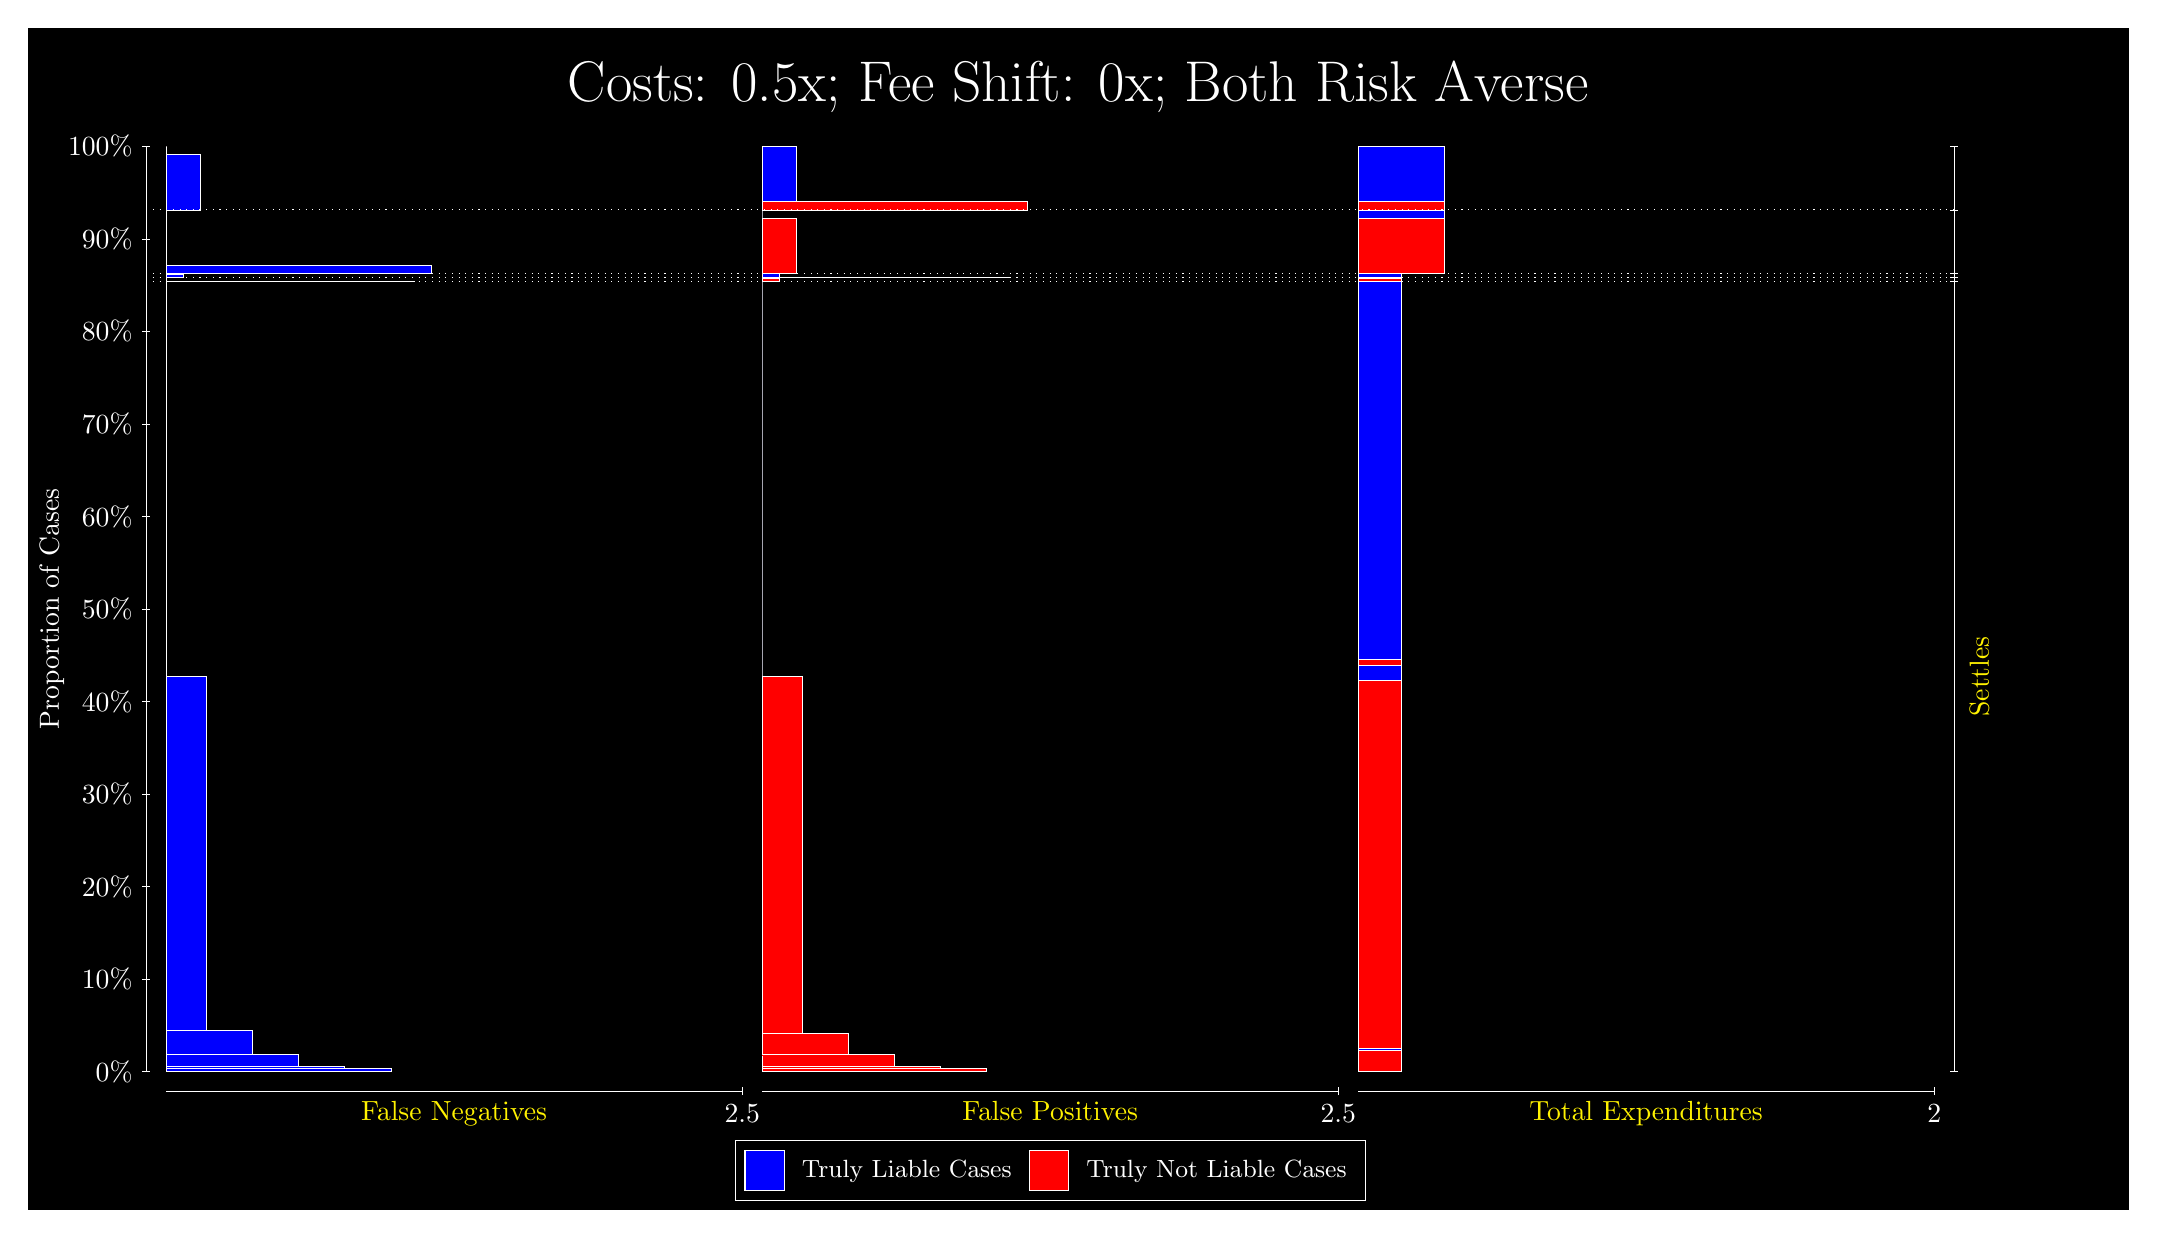
\begin{tikzpicture}
\draw[fill=black] (0,0) rectangle (26.667,15);
\draw[text=white] (0,13.5) rectangle (26.667,15) node[midway] {\huge Costs: 0.5x; Fee Shift: 0x; Both Risk Averse};
\draw[white, very thin] (1.5,1.75) -- (1.5,13.5);
\node[rotate=90, text=white, anchor=center] at (0.3, 7.625) {Proportion of Cases};
\draw[white, very thin] (1.45,1.75) -- (1.55,1.75);
\node[text=white, anchor=east] at (1.45, 1.75) {0\%};
\draw[white, very thin] (1.45,2.925) -- (1.55,2.925);
\node[text=white, anchor=east] at (1.45, 2.925) {10\%};
\draw[white, very thin] (1.45,4.1) -- (1.55,4.1);
\node[text=white, anchor=east] at (1.45, 4.1) {20\%};
\draw[white, very thin] (1.45,5.275) -- (1.55,5.275);
\node[text=white, anchor=east] at (1.45, 5.275) {30\%};
\draw[white, very thin] (1.45,6.45) -- (1.55,6.45);
\node[text=white, anchor=east] at (1.45, 6.45) {40\%};
\draw[white, very thin] (1.45,7.625) -- (1.55,7.625);
\node[text=white, anchor=east] at (1.45, 7.625) {50\%};
\draw[white, very thin] (1.45,8.8) -- (1.55,8.8);
\node[text=white, anchor=east] at (1.45, 8.8) {60\%};
\draw[white, very thin] (1.45,9.975) -- (1.55,9.975);
\node[text=white, anchor=east] at (1.45, 9.975) {70\%};
\draw[white, very thin] (1.45,11.15) -- (1.55,11.15);
\node[text=white, anchor=east] at (1.45, 11.15) {80\%};
\draw[white, very thin] (1.45,12.325) -- (1.55,12.325);
\node[text=white, anchor=east] at (1.45, 12.325) {90\%};
\draw[white, very thin] (1.45,13.5) -- (1.55,13.5);
\node[text=white, anchor=east] at (1.45, 13.5) {100\%};

\draw[white, very thin] (24.457,1.75) -- (24.457,13.5);
\draw[white, very thin] (24.407,1.75) -- (24.507,1.75);
\node[anchor=west] at (24.407, 1.75) {};
\draw[white, very thin] (24.407,11.781) -- (24.507,11.781);
\node[anchor=west] at (24.407, 11.781) {};
\draw[white, very thin] (24.407,11.834) -- (24.507,11.834);
\node[anchor=west] at (24.407, 11.834) {};
\draw[white, very thin] (24.407,11.887) -- (24.507,11.887);
\node[anchor=west] at (24.407, 11.887) {};
\draw[white, very thin] (24.407,12.694) -- (24.507,12.694);
\node[anchor=west] at (24.407, 12.694) {};
\draw[white, very thin] (24.407,13.5) -- (24.507,13.5);
\node[anchor=west] at (24.407, 13.5) {};

\draw[white, very thin, fill=blue] (1.75,1.75) rectangle (4.6044,1.7956);
\draw[white, very thin, fill=blue] (1.75,1.7956) rectangle (4.3116,1.796);
\draw[white, very thin, fill=blue] (1.75,1.796) rectangle (4.0188,1.8158);
\draw[white, very thin, fill=blue] (1.75,1.8158) rectangle (3.7261,1.8166);
\draw[white, very thin, fill=blue] (1.75,1.8166) rectangle (3.4333,1.9658);
\draw[white, very thin, fill=blue] (1.75,1.9658) rectangle (3.1406,1.9709);
\draw[white, very thin, fill=blue] (1.75,1.9709) rectangle (2.8478,2.2751);
\draw[white, very thin, fill=blue] (1.75,2.2751) rectangle (2.5551,2.2786);
\draw[white, very thin, fill=blue] (1.75,2.2786) rectangle (2.2623,6.7655);
\draw[white, very thin, fill=red] (1.75,6.7655) rectangle (1.75,11.781);
\draw[white, very thin, fill=blue] (1.75,11.781) rectangle (4.8971,11.79);
\draw[white, very thin, fill=red] (1.75,11.79) rectangle (1.75,11.834);
\draw[white, very thin, fill=blue] (1.75,11.834) rectangle (1.9696,11.879);
\draw[white, very thin, fill=red] (1.75,11.879) rectangle (1.75,11.887);
\draw[white, very thin, fill=blue] (1.75,11.887) rectangle (5.1167,11.99);
\draw[white, very thin, fill=red] (1.75,11.99) rectangle (1.75,12.694);
\draw[white, very thin, fill=blue] (1.75,12.694) rectangle (2.1891,13.398);
\draw[white, very thin, fill=red] (1.75,13.398) rectangle (1.75,13.5);
\draw[white, very thin, fill=red] (9.3189,1.75) rectangle (12.173,1.7924);
\draw[white, very thin, fill=red] (9.3189,1.7924) rectangle (11.88,1.7926);
\draw[white, very thin, fill=red] (9.3189,1.7926) rectangle (11.588,1.8156);
\draw[white, very thin, fill=red] (9.3189,1.8156) rectangle (11.295,1.8164);
\draw[white, very thin, fill=red] (9.3189,1.8164) rectangle (11.002,1.9651);
\draw[white, very thin, fill=red] (9.3189,1.9651) rectangle (10.709,1.9656);
\draw[white, very thin, fill=red] (9.3189,1.9656) rectangle (10.709,1.9691);
\draw[white, very thin, fill=red] (9.3189,1.9691) rectangle (10.417,2.2319);
\draw[white, very thin, fill=red] (9.3189,2.2319) rectangle (10.124,2.2367);
\draw[white, very thin, fill=red] (9.3189,2.2367) rectangle (9.8312,6.7659);
\draw[white, very thin, fill=blue] (9.3189,6.7659) rectangle (9.3189,11.781);
\draw[white, very thin, fill=red] (9.3189,11.781) rectangle (9.5384,11.826);
\draw[white, very thin, fill=blue] (9.3189,11.826) rectangle (9.3189,11.834);
\draw[white, very thin, fill=red] (9.3189,11.834) rectangle (12.466,11.843);
\draw[white, very thin, fill=blue] (9.3189,11.843) rectangle (9.5384,11.887);
\draw[white, very thin, fill=red] (9.3189,11.887) rectangle (9.758,12.591);
\draw[white, very thin, fill=blue] (9.3189,12.591) rectangle (9.3189,12.694);
\draw[white, very thin, fill=red] (9.3189,12.694) rectangle (12.686,12.796);
\draw[white, very thin, fill=blue] (9.3189,12.796) rectangle (9.758,13.5);
\draw[white, very thin, fill=red] (16.888,1.75) rectangle (17.437,2.0216);
\draw[white, very thin, fill=blue] (16.888,2.0216) rectangle (17.437,2.0426);
\draw[white, very thin, fill=red] (16.888,2.0426) rectangle (17.437,6.7206);
\draw[white, very thin, fill=blue] (16.888,6.7206) rectangle (17.437,6.9153);
\draw[white, very thin, fill=red] (16.888,6.9153) rectangle (17.437,6.9817);
\draw[white, very thin, fill=blue] (16.888,6.9817) rectangle (17.437,11.781);
\draw[white, very thin, fill=red] (16.888,11.781) rectangle (17.437,11.826);
\draw[white, very thin, fill=blue] (16.888,11.826) rectangle (17.437,11.834);
\draw[white, very thin, fill=red] (16.888,11.834) rectangle (17.437,11.843);
\draw[white, very thin, fill=blue] (16.888,11.843) rectangle (17.437,11.887);
\draw[white, very thin, fill=red] (16.888,11.887) rectangle (17.986,12.591);
\draw[white, very thin, fill=blue] (16.888,12.591) rectangle (17.986,12.694);
\draw[white, very thin, fill=red] (16.888,12.694) rectangle (17.986,12.796);
\draw[white, very thin, fill=blue] (16.888,12.796) rectangle (17.986,13.5);
\draw[white, dotted] (1.5,11.781) -- (24.457,11.781);
\draw[white, dotted] (1.5,11.834) -- (24.457,11.834);
\draw[white, dotted] (1.5,11.887) -- (24.457,11.887);
\draw[white, dotted] (1.5,12.694) -- (24.457,12.694);
\draw[white, very thin] (1.75,1.5) -- (9.0689,1.5);
\node[text=yellow, anchor=north] at (5.4094, 1.5) {False Negatives};
\draw[white, very thin] (9.0689,1.45) -- (9.0689,1.55);
\node[text=white, anchor=north] at (9.0689, 1.45) {2.5};

\draw[white, very thin] (9.3189,1.5) -- (16.638,1.5);
\node[text=yellow, anchor=north] at (12.978, 1.5) {False Positives};
\draw[white, very thin] (16.638,1.45) -- (16.638,1.55);
\node[text=white, anchor=north] at (16.638, 1.45) {2.5};

\draw[white, very thin] (16.888,1.5) -- (24.207,1.5);
\node[text=yellow, anchor=north] at (20.547, 1.5) {Total Expenditures};
\draw[white, very thin] (24.207,1.45) -- (24.207,1.55);
\node[text=white, anchor=north] at (24.207, 1.45) {2};

\node[text=yellow, centered, rotate=90] at (24.777, 6.7657) {Settles};





\draw (12.978300999999998,1.5) node[draw=none] (baseCoordinate) {};
\begin{scope}[align=center]
        \matrix[scale=0.5, draw=white, below=0.5cm of baseCoordinate, nodes={draw}, column sep=0.1cm]{
            \node[rectangle, draw, minimum width=0.5cm, minimum height=0.5cm, fill=blue] {}; &
            \node[draw=none, font=\small, text=white] (B) {Truly Liable Cases}; &
            \node[rectangle, draw, minimum width=0.5cm, minimum height=0.5cm, fill=red] {}; &
            \node[draw=none, font=\small, text=white] (B) {Truly Not Liable Cases}; \\
            };
\end{scope}

\end{tikzpicture}
\end{document}